%%%%%%%%%%%%%%%%%%%%%%%%%%%%%%%%%%%%%%%%%%%%%%%%%%%%%%%%%%%%%
\section{Mathematical Models}\label{sec:math_model}
%%%%%%%%%%%%%%%%%%%%%%%%%%%%%%%%%%%%%%%%%%%%%%%%%%%%%%%%%%%%%

The present work considers the dynamic interaction between an incompressible
Newtonian fluid and a deformable solid, as illustrated in
Figure~\ref{fig:fsi_problem}. At time $t$, the coupled system occupies the
moving domain
\begin{equation}
    \Omega(t) = \Omega^f(t) \cup \Omega^s(t),
\end{equation}
where $\Omega^f(t)$ and $\Omega^s(t)$ denote the fluid and solid domains,
respectively. Their boundaries are denoted by $\Gamma^f(t)$ and
$\Gamma^s(t)$, with outward-facing unit normals $\hat{\bb{n}}^f$ and
$\hat{\bb{n}}^s$. The fluid--solid interface is the common boundary
\begin{equation}
    \Gamma_\text{fsi}(t)
    =
    \Gamma^f(t) \cap \Gamma^s(t),
\end{equation}
on which the fluid and solid satisfy kinematic compatibility and dynamic
traction equilibrium.

The solid is formulated in a total Lagrangian description with respect to its
initial configuration $\Omega^s_0$, while the fluid is formulated on the
current moving domain $\Omega^f(t)$ using an arbitrary Lagrangian--Eulerian
(ALE) description. For notational compactness, the explicit time dependence of
moving domains and boundaries is omitted where no ambiguity arises.

\begin{figure}[htbp]
    \centering
    \subfigure[Initial configurations of the fluid (left) and solid (right) domains, showing the initial volumes $\Omega_0$, boundaries $\bb{\Gamma}_0$ and outward-facing unit normals $\hat{\bb{n}}_0$]
    {
        \label{fig:fsi_problem_initial}
        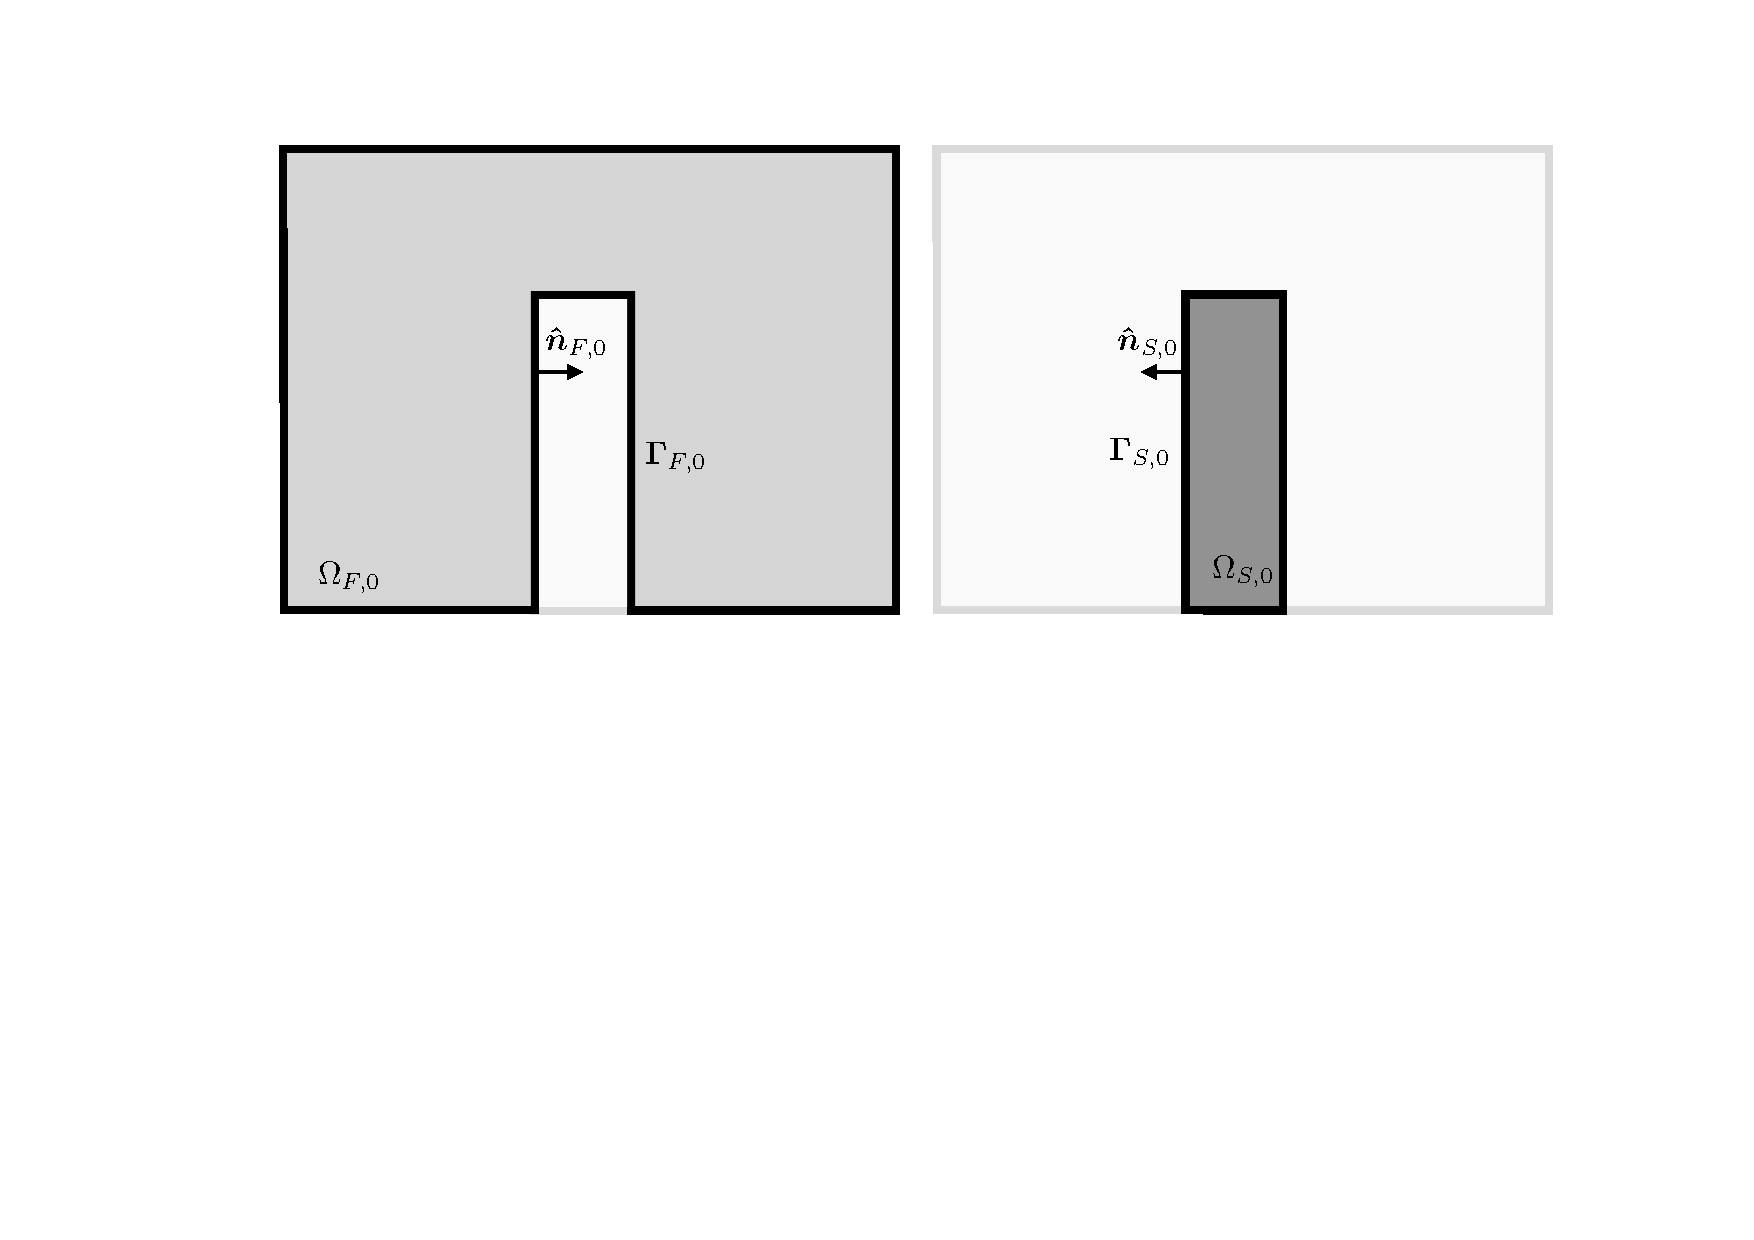
\includegraphics[width=0.8\textwidth]{figures/fsi_problem_initial}
    }
    \subfigure[Deformed configurations of the fluid (left) and solid (right) domains at time $t$, showing the deformed volumes $\Omega(t)$, boundaries $\bb{\Gamma}(t)$ and outward-facing unit normals $\hat{\bb{n}}(t)$]
    {
        \label{fig:fsi_problem_current}
        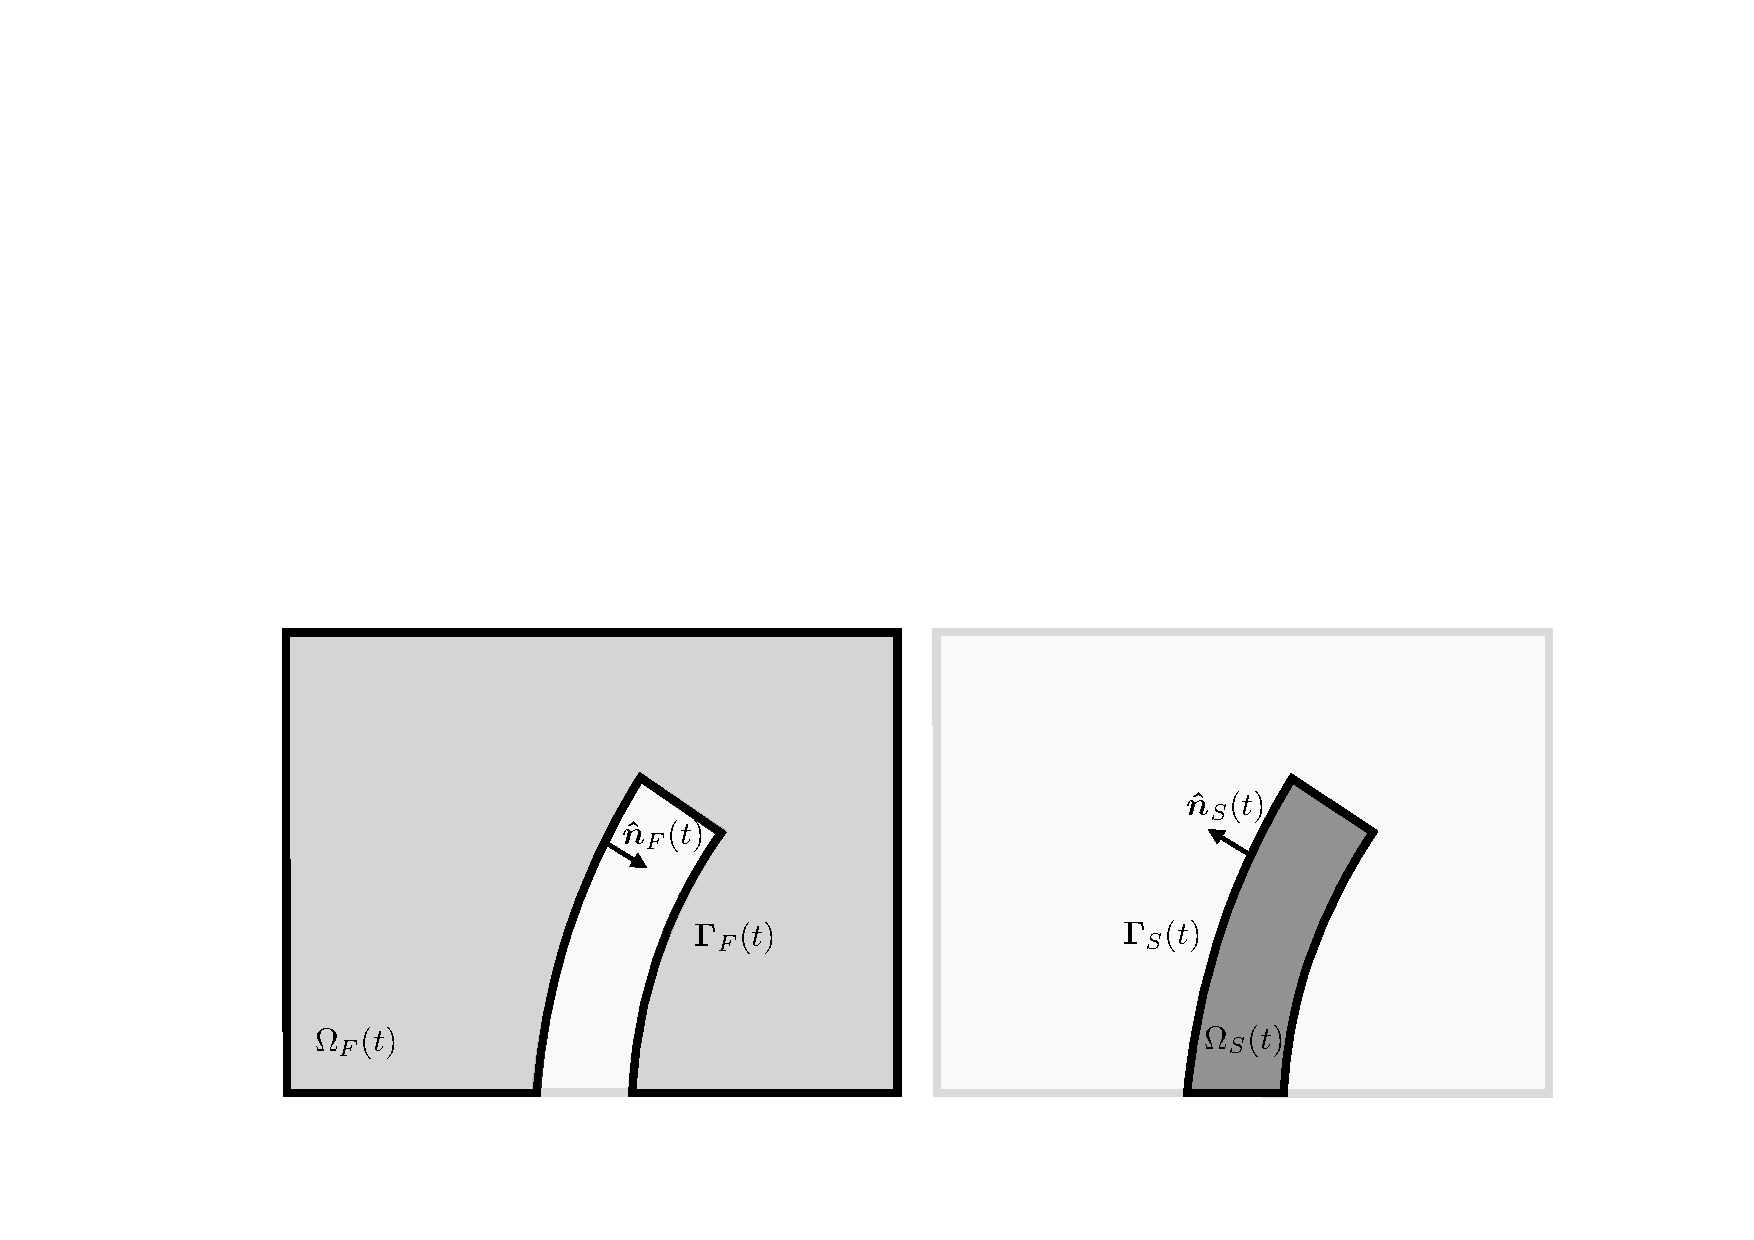
\includegraphics[width=0.8\textwidth]{figures/fsi_problem_current}
    }
    \caption{Representative fluid--solid interaction problem, where superscript $f$ represents fluid-domain quantities and superscript $s$ represents solid-domain quantities. Image adapted from \citet{OneraWebsite}.}
    \label{fig:fsi_problem}
\end{figure}


%%--------------------------------------------------------------------------------------------------------------------%%
\subsection{Solid model}
%%--------------------------------------------------------------------------------------------------------------------%%

The motion of the solid is governed by conservation of linear momentum. In the
current configuration, this may be written in integral form as
\begin{equation}
    \int_{\Omega^s}
    \rho^s
    \frac{\partial \bb{v}^s}{\partial t}
    \, d\Omega^s
    =
    \oint_{\Gamma^s}
    \hat{\bb{n}}^s \cdot \bb{\sigma}^s
    \, d\Gamma^s
    +
    \int_{\Omega^s}
    \bb{f}_b^s
    \, d\Omega^s ,
    \label{eqn:solid_momentum_current}
\end{equation}
where $\rho^s$ is the current density, $\bb{v}^s$ is the solid velocity,
$\bb{\sigma}^s$ is the true (Cauchy) stress tensor, and $\bb{f}_b^s$ is a body force
per unit current volume.

The solid equations are solved in total Lagrangian form. Let
$\bb{d}^s$ denote the solid displacement from the initial configuration
$\Omega^s_0$ to the current configuration $\Omega^s(t)$. The deformation
gradient and its determinant are
\begin{equation}
    \bb{F}
    =
    \bb{I}
    +
    \left( \bb{\nabla}_0 \bb{d}^s \right)^T,
    \qquad
    J = \det \bb{F},
    \label{eqn:deformation_gradient}
\end{equation}
where $\bb{\nabla}_0$ denotes differentiation with respect to the initial
solid coordinates. With the convention
$(\nabla_0 d^s)_{ij} = \partial d^s_j / \partial X_i$, this corresponds in
index notation to
\begin{equation}
    F_{ij}
    =
    \delta_{ij}
    +
    \frac{\partial d^s_i}{\partial X_j}.
\end{equation}

Using Nanson's relation,
\begin{equation}
    \hat{\bb{n}}^s \, d\Gamma^s
    =
    J \bb{F}^{-T} \cdot \hat{\bb{n}}^s_0 \, d\Gamma^s_0,
\end{equation}
the solid momentum equation may be expressed over the initial configuration as
\begin{equation}
    \int_{\Omega^s_0}
    \rho^s_0
    \frac{\partial^2 \bb{d}^s}{\partial t^2}
    \, d\Omega^s_0
    =
    \oint_{\Gamma^s_0}
    \left(
    J \bb{F}^{-T} \cdot \hat{\bb{n}}^s_0
    \right)
    \cdot
    \bb{\sigma}^s
    \, d\Gamma^s_0
    +
    \int_{\Omega^s_0}
    \bb{f}_{b0}^s
    \, d\Omega^s_0 .
    \label{eqn:solid_momentum_TL}
\end{equation}
Here $\rho^s_0$ is the initial density and $\bb{f}_{b0}^s$ is a body force per
unit initial volume. The true (Cauchy) stress $\bb{\sigma}^s$ is supplied by the chosen
mechanical law. In this work, the considered mechanical laws include linear
elasticity and the hyperelastic laws described in Appendix~A of \citet{Cardiff2025JFNK}.
\hl{UPDATE: we should at least state the names of the laws we use - do this when the test cases are all defined}

The solid boundary conditions considered are prescribed displacement,
prescribed traction, and symmetry conditions.


%%--------------------------------------------------------------------------------------------------------------------%%
\subsection{Fluid model}
\label{sec:fluid_governing_eqn}
%%--------------------------------------------------------------------------------------------------------------------%%

The fluid is modelled as laminar, incompressible, Newtonian and isothermal. It
is formulated on the current moving domain $\Omega^f(t)$ using an arbitrary
Lagrangian--Eulerian (ALE) description. Let $\bb{v}^f$ denote the fluid velocity
and let $\bb{v}^{\Gamma}$ denote the velocity of the moving fluid domain. The
motion of $\Omega^f(t)$ is prescribed on the fluid--solid interface by the
kinematic condition in Section~\ref{sec:fsi_interface}; its extension into the
interior of the fluid domain is a numerical mesh-motion procedure described in
Section~\ref{sec:numerical_method}.

For an incompressible fluid, conservation of mass over a moving control volume
may be written as
\begin{equation}
    \frac{d}{dt}
    \int_{\Omega^f}
    d\Omega^f
    +
    \oint_{\Gamma^f}
    \hat{\bb{n}}^f
    \cdot
    \left(
    \bb{v}^f - \bb{v}^{\Gamma}
    \right)
    \, d\Gamma^f
    =
    0 .
    \label{eqn:fluid_continuity_ale_full}
\end{equation}

The moving domain is required to satisfy the geometric conservation law,
\begin{equation}
    \frac{d}{dt}
    \int_{\Omega^f}
    d\Omega^f
    -
    \oint_{\Gamma^f}
    \hat{\bb{n}}^f
    \cdot
    \bb{v}^{\Gamma}
    \, d\Gamma^f
    =
    0 ,
    \label{eqn:gcl}
\end{equation}
so that Equation~\eqref{eqn:fluid_continuity_ale_full} is equivalent to
\begin{equation}
    \oint_{\Gamma^f}
    \hat{\bb{n}}^f
    \cdot
    \bb{v}^f
    \, d\Gamma^f
    =
    0 .
    \label{eqn:fluid_continuity_ale}
\end{equation}

%In the finite-volume discretisation, this condition is enforced through the
%discrete velocity fluxes, with the mesh-motion contribution treated through the
%ALE relative flux.

Conservation of linear momentum in ALE form is written as
\begin{equation}
    \frac{d}{dt}
    \int_{\Omega^f}
    \bb{v}^f
    \, d\Omega^f
    +
    \oint_{\Gamma^f}
    \hat{\bb{n}}^f
    \cdot
    \left(
    \bb{v}^f - \bb{v}^{\Gamma}
    \right)
    \bb{v}^f
    \, d\Gamma^f
    =
    \oint_{\Gamma^f}
    \hat{\bb{n}}^f
    \cdot
    \bb{\sigma}^f
    \, d\Gamma^f
    +
    \int_{\Omega^f}
    \bb{f}_b^f
    \, d\Omega^f ,
    \label{eqn:fluid_momentum_ale}
\end{equation}
where $\bb{f}_b^f$ is a body force per unit mass. The use of a kinematic
pressure gives the Newtonian stress tensor
\begin{equation}
    \bb{\sigma}^f
    =
    \nu
    \left[
    \bb{\nabla} \bb{v}^f
    +
    \left( \bb{\nabla} \bb{v}^f \right)^T
    \right]
    -
    p \bb{I},
    \label{eqn:fluid_stress}
\end{equation}
where $\nu$ is the kinematic viscosity and $p$ is the kinematic pressure.

The fluid boundary conditions considered are inlet, outlet, no-slip wall and
symmetry conditions. On the fluid--solid interface, the fluid velocity is
constrained by the solid velocity through the kinematic interface condition
defined in Section~\ref{sec:fsi_interface}.


%%--------------------------------------------------------------------------------------------------------------------%%
\subsection{Interface conditions}
\label{sec:fsi_interface}
%%--------------------------------------------------------------------------------------------------------------------%%

The fluid and solid are coupled by kinematic and dynamic conditions on the
fluid--solid interface $\Gamma_\text{fsi}(t)$. The kinematic condition enforces
continuity of velocity between the fluid and solid and also prescribes the
motion of the fluid-domain boundary:
\begin{equation}
    \bb{v}^f
    =
    \bb{v}^s
    =
    \bb{v}^{\Gamma}
    =
    \frac{\partial \bb{d}^s}{\partial t}
    \qquad
    \text{on } \Gamma_\text{fsi}(t),
    \label{eqn:kinematic_interface}
\end{equation}
where $\bb{v}^{\Gamma}$ is the velocity of the moving fluid domain. This condition
prevents slip, gap formation and overlap at the interface. Away from the
interface, the extension of the boundary motion into the fluid domain is a
numerical mesh-motion procedure and is described in
Section~\ref{sec:numerical_method}.

The dynamic condition enforces equilibrium of the fluid and solid tractions,
\begin{equation}
    \bb{t}^f
    +
    \bb{t}^s
    =
    \bb{0}
    \qquad
    \text{on } \Gamma_\text{fsi}(t),
    \label{eqn:dynamic_interface_compact}
\end{equation}
with
\begin{equation}
    \bb{t}^f
    =
    \hat{\bb{n}}^f \cdot \bb{\sigma}^f,
    \qquad
    \bb{t}^s
    =
    \hat{\bb{n}}^s \cdot \bb{\sigma}^s,
    \qquad
    \hat{\bb{n}}^f = -\hat{\bb{n}}^s .
\end{equation}
Equivalently,
\begin{equation}
    \hat{\bb{n}}^f \cdot \bb{\sigma}^f
    =
    -
    \hat{\bb{n}}^s \cdot \bb{\sigma}^s
    \qquad
    \text{on } \Gamma_\text{fsi}(t).
    \label{eqn:dynamic_interface}
\end{equation}

%Using Equation~\eqref{eqn:fluid_stress}, the fluid traction is
%\begin{equation}
%    \bb{t}^f
%    =
%    \hat{\bb{n}}^f
%    \cdot
%    \left\{
%    \nu
%    \left[
%    \bb{\nabla} \bb{v}^f
%    +
%    \left( \bb{\nabla} \bb{v}^f \right)^T
%    \right]
%    -
%    p \bb{I}
%    \right\}.
%    \label{eqn:fluid_interface_traction}
%\end{equation}

%In the implemented formulation, the traction passed from the fluid to the solid
%may contain either the pressure contribution alone or the full fluid traction,
%including the viscous contribution. Unless otherwise stated, the calculations
%reported in this work transfer both pressure and viscous tractions.


%%%--------------------------------------------------------------------------------------------------------------------%%
%\subsection{Fluid mesh motion}
%\label{sec:fluid_domain_motion}
%%%--------------------------------------------------------------------------------------------------------------------%%
%
%The ALE fluid formulation requires the motion of the fluid mesh to be specified.
%The mesh motion is not a physical conservation law; rather, it is an auxiliary
%problem used to propagate the interface displacement smoothly into the fluid
%domain while maintaining mesh quality.
%
%Let $\bb{d}^{\Gamma}$ denote the fluid mesh displacement. On the fluid--solid
%interface, the mesh displacement is prescribed from the solid displacement,
%\begin{equation}
%    \bb{d}^{\Gamma}
%    =
%    \bb{d}^s
%    \qquad
%    \text{on } \Gamma_\text{fsi}(t),
%    \label{eqn:mesh_motion_interface_bc}
%\end{equation}
%while appropriate prescribed or symmetry conditions are applied on the remaining
%fluid boundaries.
%
%In this work, the fluid mesh displacement is computed using a pseudo-solid
%linear-elasticity equation,
%\begin{equation}
%    \oint_{\Gamma^f_0}
%    \hat{\bb{n}}^f_0
%    \cdot
%    \left[
%    \mu^\Gamma
%    \bb{\nabla}_0 \bb{d}^{\Gamma}
%    +
%    \mu^\Gamma
%    \left(
%    \bb{\nabla}_0 \bb{d}^{\Gamma}
%    \right)^T
%    +
%    \lambda^\Gamma
%    \left(
%    \bb{\nabla}_0 \cdot \bb{d}^{\Gamma}
%    \right)
%    \bb{I}
%    \right]
%    \, d\Gamma^f_0
%    =
%    \bb{0}.
%    \label{eqn:mesh_motion_pseudo_solid}
%\end{equation}
%The coefficients $\mu^\Gamma$ and $\lambda^\Gamma$ are artificial stiffness
%parameters used only to control the distribution of mesh motion. They are
%spatially varied so that the mesh is stiffer near the fluid--solid interface;
%in the present implementation, the stiffness is scaled inversely with the
%square of the distance from the interface. This reduces mesh distortion near
%the moving boundary while allowing the displacement to decay smoothly into the
%fluid domain.
%
%The mesh velocity is then obtained from the time derivative of
%$\bb{d}^{\Gamma}$ and used in the ALE fluxes in
%Equations~\eqref{eqn:fluid_continuity_ale_full} and
%\eqref{eqn:fluid_momentum_ale}. The discrete moving-mesh fluxes are constructed
%so as to satisfy the geometric conservation law,
%Equation~\eqref{eqn:gcl}.
